\documentclass[12pt]{article}
\usepackage[english]{babel}
\usepackage[utf8]{inputenc} % Permite el uso de caracteres del Español
\usepackage[T1]{fontenc}
\usepackage{graphicx}
\usepackage{amsmath}
\usepackage{wrapfig}
\usepackage{enumerate}
\usepackage[top=1in, bottom=1.25in, left=1.1in, right=1.1in]{geometry}
\usepackage[dvipsnames]{xcolor}
\usepackage{subcaption}

\begin{document}

\begin{titlepage}

\newcommand{\HRule}{\rule{\linewidth}{0.5mm}} % Define un comando para las lineas horizontales

\center 
%----------------------------------------------------------------------------------------
%	Cabezera
%----------------------------------------------------------------------------------------

\textsc{\LARGE Universidad de Sonora}\\[1.5cm]
\textsc{\Large Licenciatura en Física}\\[0.5cm]
\textsc{\large Física Computacional I}\\[0.5cm]

%----------------------------------------------------------------------------------------
%	Titulo
%----------------------------------------------------------------------------------------

\HRule \\[0.4cm]
{\huge \bfseries Actividad 3 - Sondeos meteorológicos de la Atmósfera}\\[0.4cm] % Title of your document
\HRule \\[1.5cm]
 
%----------------------------------------------------------------------------------------
%	Autor
%----------------------------------------------------------------------------------------

\begin{minipage}{0.4\textwidth}
\begin{flushleft} \large
\emph{Alumno:}\\
José Gabriel Navarro I.
\end{flushleft}
\end{minipage}
~
\begin{minipage}{0.4\textwidth}
\begin{flushright} \large
\emph{Profesor:} \\
Carlos Lizarraga Celaya
\end{flushright}
\end{minipage}\\[2cm]


%----------------------------------------------------------------------------------------
%	Fecha
%----------------------------------------------------------------------------------------
14 de Febrero de 2018

%----------------------------------------------------------------------------------------
%	Escudo
%----------------------------------------------------------------------------------------


\includegraphics[width=0.4\textwidth]{logo.png}\\
 
%----------------------------------------------------------------------------------------

\vfill % Llena el espacio de la pagina en blanco

\end{titlepage}

\section{Introducción}
En el presente reporte se habla acerca de la tercera actividad realizada para la clase de Física Computacional I, el cual abarca un análisis de datos acerca de varias características de la atmósfera revisando variaciones de distintas propiedades con respecto a la altura. \\

Primeramente se habla acerca de los fundamentos de la investigación, en donde se habla un poco acerca de lo ya investigado anteriormente de la atmósfera terrestre y sus propiedades. Posteriormente se habla acerca del análisis de datos, y el proceso que se tuvo que realizar para poder analizar los datos deseados. Estos datos se tomaron del Observatorio de Valentia, ubicado en la isla de Valentia. Una vez que analizamos los datos, se presentan los resultados de este análisis, en donde se pueden encontrar gráficas de distintas variables con respecto a la altura, y su interpretación. Al final se presenta una conclusión de la actividad, así como la bibliografía utilizada para la investigación de los fundamentos y el apéndice. 

\section{Fundamentos}
Como se había hablado en practicas anteriores, la atmósfera consiste en 5 capas:     Troposfera, Estratosfera, Mesosfera, Termosfera y Exosfera. \\

La troposfera es la capa mas baja de la atmósfera terrestre y se extiende desde la superficie de la Tierra, donde su altura depende del lugar y varia entre los 9 km hasta los 17 km en el ecuador. Aunque si ocurren variaciones, la temperatura usualmente declina con el aumento de altitud, ya que esta capa esta siendo calentada por la transferencia de energía de la superficie pero se detiene al llegar a una capa llamada tropopausa. Aquí es donde se ubica la corriente en chorro, y donde casi todo el vapor de agua o humedad esta contenida, por lo cual define el punto más alto donde pueden suceder los fenómenos meteorológicos. \\

Las siguientes capas también su temperatura depende de la altitud a la que nos encontramos. En la estratosfera el aumento en temperatura es causado por la absorción de la radiación ultravioleta y a pesar de que la temperatura en la tropopausa es alrededor de -60 $^{\circ}$C, en la parte superior de la estratosfera es 0 $^{\circ}$C. La mesosfera, la siguiente capa, sus temperaturas (igual que antes) bajan cuando aumenta la altitud, por lo cual es el lugar mas helado de la Tierra, su temperatura media esta entre los -85 $^{\circ}$C. Y la capa mas externa, la termosfera, su temperatura aumenta ya que recibe directamente la radiación solar. \\ 

Es por eso que en este reporte se presenta el análisis de propiedades físicas y estado de la atmósfera durante el día, dependiendo de la altura en la que se encuentra. 

\section{Análisis de datos}
Primeramente, se recuperaron los datos de dos días distintos, en estaciones del año distintas. Se tomaron datos del Observatorio de Valentia, en los días 22 de Diciembre de 2017, y 22 de Junio de 2017. Como se puede observar, estamos tomando datos en distintas estaciones, siendo estas Invierno y Verano respectivamente. Este lapso entre estaciones nos permite analizar los cambios de temperatura, velocidad de vientos, humedad entra otras propiedades dependiendo de nuestro clima. \\

La información se obtuvo del sitio de sondeos atmosféricos de la Universidad de Wyoming. En donde se selecciono la estación del Observatorio de Valentia. Los datos fueron guardados en un archivo txt siendo su formato de la siguiente forma:

\begin{center}
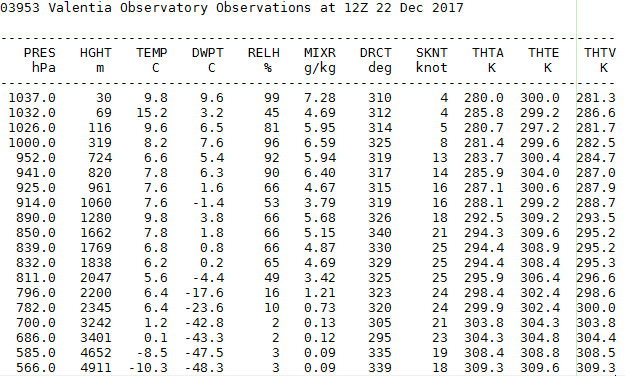
\includegraphics[scale=0.7]{Datos.png}
\end{center}

Debido a que se tiene una cabecera con datos innecesarios como lo es el titulo y las unidades, nos pasamos esas lineas al leer los datos, ademas de eliminar el ultimo renglón de símbolos. Ademas de esto en el archivo vienen datos adicionales al final de los datos que tampoco necesitamos, así que los eliminamos también. 

\begin{center}
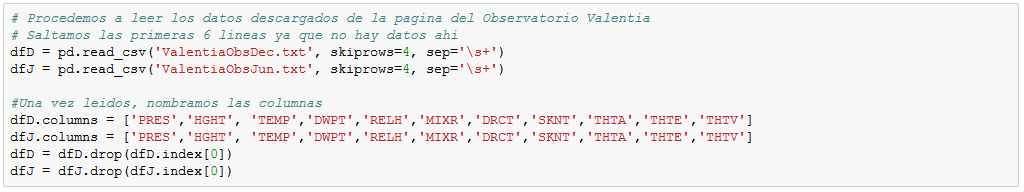
\includegraphics[scale=0.65]{AnaDatos.png}
\end{center}

\begin{center}
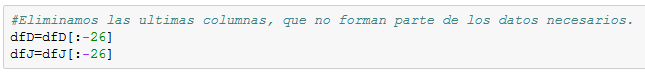
\includegraphics[scale=0.65]{Elim.png}
\end{center}

El resultado que se obtiene es el siguiente:

\begin{center}
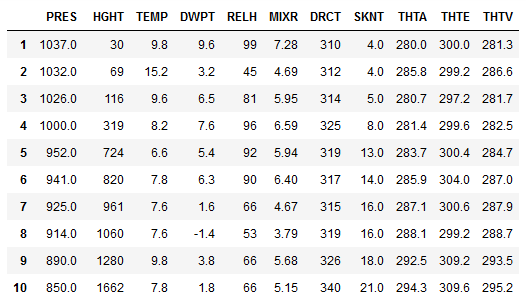
\includegraphics[scale=0.65]{AnaDatosResul.png}
\end{center}

Posteriormente, se cambiaron el tipo de datos del dataframe, ya que algunos de ellos fueron tomados como objeto. Los tomamos a todos en una sola variable y los pasamos a numéricos. De esta manera ya podemos utilizar estos datos para graficar. 

\begin{center}
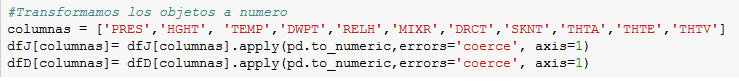
\includegraphics[scale=0.65]{Cambia.png}
\end{center}

\section{Resultados}
A continuación se presentan las graficas de las distintas comparaciones entre la altura y otras propiedades, siendo estas las indicadas en la actividad. \\

\noindent\textbf{Producir una gráfica de la variación de la presión con respecto a la altura}
\begin{figure}[h!]
\begin{subfigure}{.55\textwidth}
  \centering
  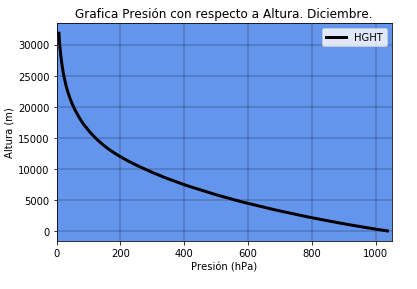
\includegraphics[width=.8\linewidth]{GrafAPDec.png}
  \caption{Análisis de Diciembre}
  \label{fig:sfig1}
\end{subfigure}
\begin{subfigure}{.55\textwidth}
  \centering
  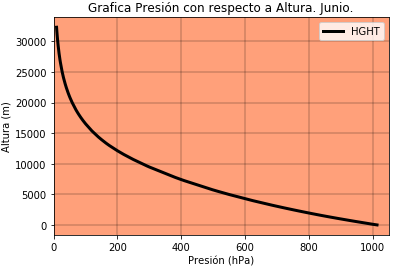
\includegraphics[width=.8\linewidth]{GrafAPJun.png}
  \caption{Análisis de Junio}
  \label{fig:sfig2}
\end{subfigure}
\end{figure}

Como se puede observar en las graficas,  se cumple lo que se ha investigado anteriormente. Cuando la altura aumenta, la presión va disminuyendo hasta llegar a casi cero, además también se puede notar que no hay mucho cambio debido a ser estaciones distintas. \\

\noindent\textbf{Hacer una gráfica de temperatura como función de la altura. ¿Hay cambios significativos en la tropopausa entre las dos fechas?} 

\begin{figure}[h!]
\begin{subfigure}{.55\textwidth}
  \centering
  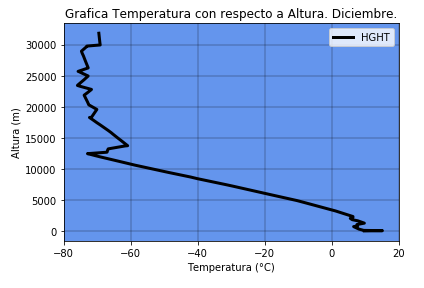
\includegraphics[width=.8\linewidth]{GrafATDec.png}
  \caption{Análisis de Diciembre}
  \label{fig:sfig1}
\end{subfigure}
\begin{subfigure}{.55\textwidth}
  \centering
  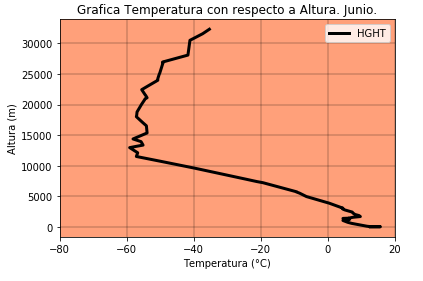
\includegraphics[width=.8\linewidth]{GrafATJun.png}
  \caption{Análisis de Junio}
  \label{fig:sfig2}
\end{subfigure}
\end{figure}

En Diciembre la temperatura baja hasta a -75$^{\circ}$C a una altura de aproximadamente 12.5 km. Sin embargo, en Junio a esa misma distancia, la temperatura llega hasta -60$^{\circ}$C. Sin embargo, la tropopausa se encuentra aproximadamente a 10km de la Tierra, entre la troposfera y la estratosfera. Como se puede observar, el cambio también es notable a esta altura, donde la temperatura en diciembre es de aproximadamente -55$^{\circ}$C, mientras que en Junio es de -35$^{\circ}$C. \\

\noindent\textbf{Gráfica de la temperatura (TEMP) y temperatura de rocío (DEWPT), como función de la altura.} \\

La temperatura de rocío es la más baja temperatura a la que empieza a condensarse el vapor de agua contenido en el aire, produciendo rocío, neblina, cualquier tipo de nube o, en caso de que la temperatura sea lo suficientemente baja, escarcha. 

\begin{figure}[h!]
\begin{subfigure}{.55\textwidth}
  \centering
  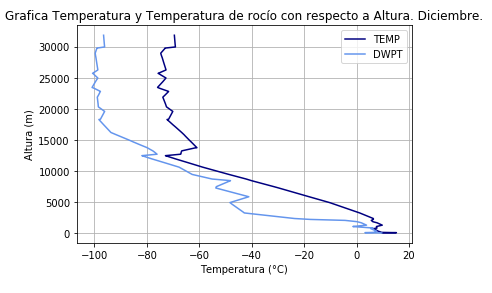
\includegraphics[width=.8\linewidth]{GrafATTDec.png}
  \caption{Análisis de Diciembre}
  \label{fig:sfig1}
\end{subfigure}
\begin{subfigure}{.55\textwidth}
  \centering
  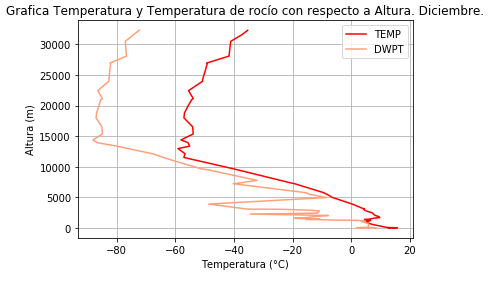
\includegraphics[width=.8\linewidth]{GrafATTJun.png}
  \caption{Análisis de Junio}
  \label{fig:sfig2}
\end{subfigure}
\end{figure}

Como podemos observar en ambas graficas y ya se ha mencionado, entre mas altura hay, la temperatura aumenta, sin embargo, como se puede notar, la temperatura de rocío siempre es mas baja que la temperatura normal, ya que por su descripción, esta es la temperatura mas baja en la que empieza a condensarse el vapor de agua. Otra cosa que es importante mencionar, es que dependiendo de la estación la temperatura es afectada, haciendo que en verano sea mayor a que la de invierno. Además, el patrón que sigue la temperatura y la temperatura de rocío son muy parecidas. \\

\noindent\textbf{Gráfica de la rapidez de los vientos en nudos (SKNT).} 
\begin{figure}[h!]
\begin{subfigure}{.55\textwidth}
  \centering
  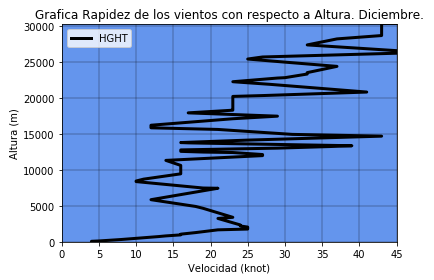
\includegraphics[width=.8\linewidth]{GrafAVDec.png}
  \caption{Análisis de Diciembre}
  \label{fig:sfig1}
\end{subfigure}
\begin{subfigure}{.55\textwidth}
  \centering
  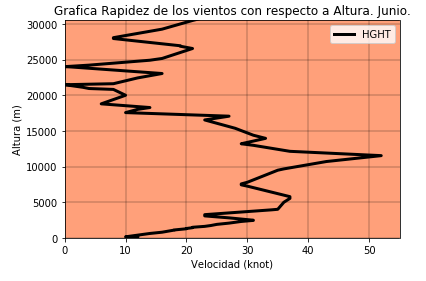
\includegraphics[width=.8\linewidth]{GrafAVJun.png}
  \caption{Análisis de Junio}
  \label{fig:sfig2}
\end{subfigure}
\end{figure}

Los vientos en nudos hacen referencia a la velocidad de los vientos dependiendo de la altura, y con nudo se refiere a la unidad para medir la velocidad de estos. Un nudo es equivalente a  1.852 m/h (metros por hora). Gráficamente podemos observar como entre mas altura, mayor va a ser la velocidad de los vientos, esto se puede explicar ya que los vientos se originan como consecuencia de las diferencias en la presión atmosférica y estas diferencias se producen por las distintas temperaturas en el aire. Entonces entre mayor sea la diferencia, mayor sera la velocidad. \\

\noindent\textbf{Gráfica de la humedad relativa como función de la altura.}
\noindent\textbf{Gráfica de la rapidez de los vientos en nudos (SKNT).} 
\begin{figure}[h!]
\begin{subfigure}{.55\textwidth}
  \centering
  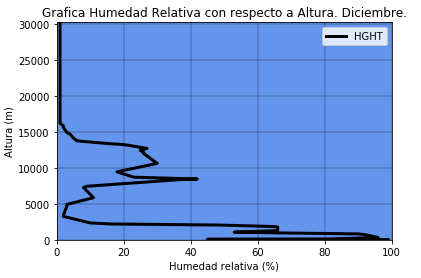
\includegraphics[width=.8\linewidth]{GrafAHDec.png}
  \caption{Análisis de Diciembre}
  \label{fig:sfig1}
\end{subfigure}
\begin{subfigure}{.55\textwidth}
  \centering
  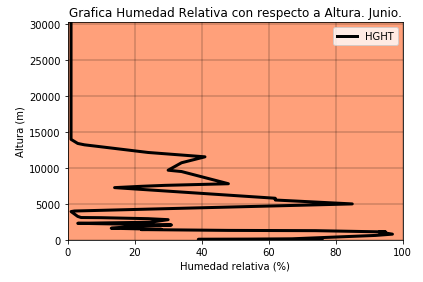
\includegraphics[width=.8\linewidth]{GrafAHJun.png}
  \caption{Análisis de Junio}
  \label{fig:sfig2}
\end{subfigure}
\end{figure}

La humedad relativa es el porcentaje de la humedad de saturación, que se calcula normalmente en relación con la densidad de vapor de saturación. Se puede observar gráficamente que el porcentaje es alto cuando estamos a alturas bajas pero cuando empieza a aumentar la altura hay una gran caída a porcentajes pequeños, llegando hasta a 1\% después de los 15,000 m. Entre los 10,000 m y 15,000 m podemos observar una aumento en porcentaje, siendo mayor en el verano.

\section{Conclusión}
Después del análisis y limpieza de estos datos, pude concluir que mas que graficar, el trabajo del análisis de datos reside en la limpieza de estos. Como se menciono en el apartado de análisis de datos, se tuvieron que realizar distintos procesos para poder utilizarlos y hacer las respectivas graficas, se tuvo que eliminar la cabecera, renombrar las columnas, eliminar la información debajo de los datos, y cambiar en algunos casos el tipo de dato a las columnas de datos. \\

Con esto queda en claro que el analizar datos no es simplemente tomar una lista de datos, graficarlos y analizarlos. Importa también su limpieza y cuidado, así como también poder realizar dicha limpieza y cuidado de la manera mas eficiente y rápida, porque si tenemos que analizar 500 archivos, y nos ponemos a revisar manualmente cada uno de ellos, tomaría mucho tiempo a que si lo hiciéramos con panda y Python.

\section{Bibliografía}
\begin{itemize}
    \item Atmosphere of Earth. (2018, Enero 24). Recuperado de: en.wikipedia.org/wiki \\ /Atmosphere\_of\_Earth
    \item Las 5 capas de la atmosfera. (2017, Mayo 8). Recuperado de: www.meteorologiaenred.com/capas-atmosfera.html
    \item Punto de rocío. (2018, Enero 18). Recuperado de: es.wikipedia.org/wiki/Punto\_de\_\\roc\%C3\%ADo
    \item Relative Humidity. Recuperado de: http://hyperphysics.phy-astr.gsu.edu/hbasees/\\Kinetic/relhum.html
\end{itemize}

\section{Apéndice}
\noindent\textbf {1. ¿Cuál es tu opinión general de esta actividad?} \\ \\
Esta actividad permitió desarrollar mas lo que viene siendo el análisis de datos y su posterior gráfica, algo que será indispensable en el curso, por lo cual es una buena practica. Como ya se había mencionado en clase, se invierte mas tiempo limpiando los datos que haciendo la gráfica, por lo cual es muy importante aprender a realizar esta limpieza.  \\ \\

\noindent\textbf {2. ¿Qué fue lo que más te agradó? ¿Lo que menos te agradó?}\\ \\
Me gusto investigar como limpiar un archivo y posteriormente graficar los datos con distintos formatos dependiendo del mes, le da una buena organización a todo y me quede satisfecho con el trabajo. Lo que menos me agrado fue la confusión al almacenar el archivo de los datos, ya que la pagina no respondía bien y tarde un poco en entender como funcionaba. \\ 

\noindent\textbf {3. ¿Qué consideras que aprendiste en esta actividad? } \\ \\
Mejore en la lectura de archivos mediante la librería panda y aprendí a utilizar de una mejor manera las gráficas utilizando la librería matplotlib, dando color y distinguiendo entre las distintas gráficas. \\

\noindent\textbf {4. ¿Qué le faltó? ¿O le sobró?  } \\ \\
Siento que falto una introducción a la práctica, una idea general de lo que se tiene que hacer. Las instrucciones de la página a veces se pueden malinterpretar y puede terminar en resultados erróneos. \\

\noindent\textbf {5. ¿Qué mejoras sugieres a la actividad?}\\  \\
Un lugar en donde se pueda descargar mas fácilmente la información a utilizar.
\end{document}